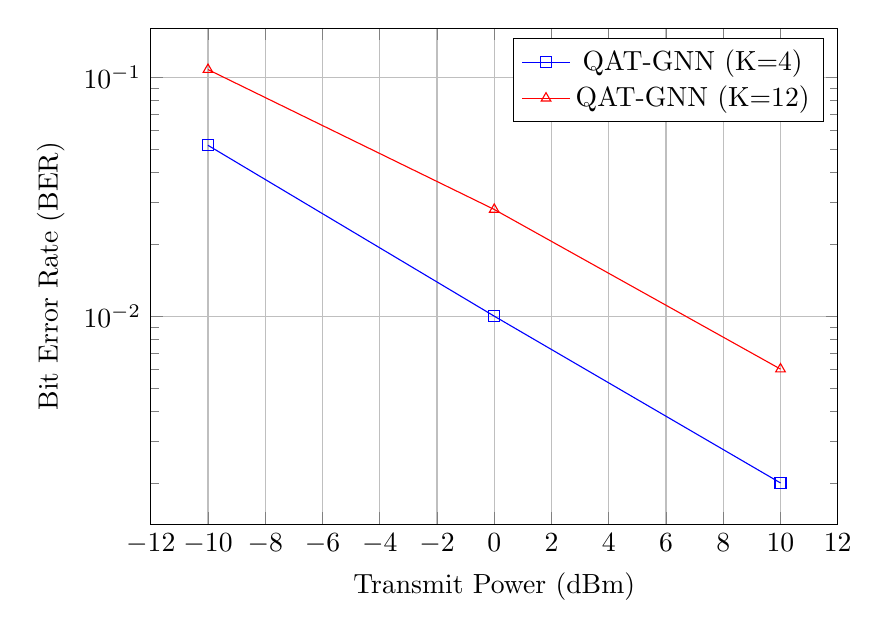
\begin{tikzpicture}
\begin{semilogyaxis}[
    xlabel={Transmit Power (dBm)},
    ylabel={Bit Error Rate (BER)},
    grid=major,
    width=0.85\linewidth,
    height=0.65\linewidth,
    legend style={at={(0.98,0.98)},anchor=north east}
]
\addplot[color=blue, mark=square] coordinates {(-10, 0.052) (0, 0.010) (10, 0.002)}; \addlegendentry{QAT-GNN (K=4)}
\addplot[color=red, mark=triangle] coordinates {(-10, 0.108) (0, 0.028) (10, 0.006)}; \addlegendentry{QAT-GNN (K=12)}
\end{semilogyaxis}
\end{tikzpicture}